% ============================================================
% LLM-BLM 補足実験 X05（探索）：見通しの大きさ（alpha）の倍率と、LLM・NLP の点数ごとの月次の BLM
% コンパイル：tectonic -X compile LLM-BLM_補足実験_αの大きさ.tex   （XeTeX 系。このフォルダで実行する）
% 図は 図/（作成スクリプト/figs.py が experiments/X05_alpha_scale/results から作る）
% ============================================================
\documentclass[xelatex,ja=standard,jafont=haranoaji,a4paper,10pt,openany]{bxjsreport}
\setpagelayout*{left=24mm,right=24mm,top=24mm,bottom=26mm,footskip=11mm}

\usepackage{amsmath,amssymb,mathtools,bm}
\usepackage{booktabs,array,multirow,longtable}
\usepackage{graphicx}
\usepackage{adjustbox}
\usepackage{xcolor}
\usepackage{tikz}
\usetikzlibrary{arrows.meta,positioning,calc,fit}
\usepackage{enumitem}
\usepackage{caption}
\usepackage{float}
\usepackage[most]{tcolorbox}
\usepackage[hidelinks,bookmarksnumbered]{hyperref}
\pdfstringdefDisableCommands{\def\Omega{Ω}\def\tau{τ}\def\Sigma{Σ}}

\graphicspath{{図/}}

\definecolor{c1}{HTML}{2A78D6}
\definecolor{c2}{HTML}{EB6834}
\definecolor{c3}{HTML}{1BAF7A}
\definecolor{c4}{HTML}{EDA100}
\definecolor{c7}{HTML}{6250D6}
\definecolor{ink2}{HTML}{52514E}
\definecolor{soft1}{HTML}{E4EEF9}
\definecolor{soft2}{HTML}{FBEEDF}
\definecolor{soft3}{HTML}{E3F3E9}
\definecolor{soft4}{HTML}{EEE8FA}
\definecolor{soft5}{HTML}{FDF3DA}

\newcommand{\code}[1]{\texttt{#1}}
\newcommand{\SP}{S\&P500}
\newcommand{\figref}[1]{図~\ref{#1}}
\newcommand{\tabref}[1]{表~\ref{#1}}
\newcommand{\chapref}[1]{第~\ref{#1}~章}
\newcommand{\secref}[1]{\ref{#1}~節}

\setlist[itemize]{leftmargin=1.6em,itemsep=0.2em,topsep=0.4em}
\setlist[enumerate]{leftmargin=1.8em,itemsep=0.2em,topsep=0.4em}
\captionsetup{font=small,labelfont=bf,skip=6pt}
\renewcommand{\arraystretch}{1.2}
\setlength{\LTpre}{6pt}
\setlength{\LTpost}{6pt}

\makeatletter
\def\@makechapterhead#1{\vspace*{0.3\Cvs}{\parindent\z@\raggedright\normalfont
  \ifnum\c@secnumdepth>\m@ne\if@mainmatter{\Large\headfont\@chapapp\thechapter\@chappos}\par\nobreak\vskip0.4\Cvs\fi\fi
  \interlinepenalty\@M\LARGE\headfont #1\par\nobreak\vskip 1.5\Cvs}}
\def\@makeschapterhead#1{\vspace*{0.3\Cvs}{\parindent\z@\raggedright\normalfont
  \interlinepenalty\@M\LARGE\headfont #1\par\nobreak\vskip 1.5\Cvs}}
\makeatother

\newtcolorbox{keybox}[1][要点]{enhanced,breakable,colback=soft1,colframe=c1,boxrule=0.5pt,arc=2pt,
  left=8pt,right=8pt,top=6pt,bottom=6pt,title={#1},fonttitle=\sffamily\bfseries\small,coltitle=white}
\newtcolorbox{notebox}[1][注意]{enhanced,breakable,colback=soft2,colframe=c2,boxrule=0.5pt,arc=2pt,
  left=8pt,right=8pt,top=6pt,bottom=6pt,title={#1},fonttitle=\sffamily\bfseries\small,coltitle=white}
\newtcolorbox{verdict}[1][判定]{enhanced,breakable,colback=soft4,colframe=c7,boxrule=0.5pt,arc=2pt,
  left=8pt,right=8pt,top=6pt,bottom=6pt,title={#1},fonttitle=\sffamily\bfseries\small,coltitle=white}

\tikzset{
  box/.style={draw=#1,fill=#1!8,rounded corners=2pt,align=center,font=\footnotesize,inner sep=4pt,
              minimum height=10mm,text width=24mm},
  arr/.style={-{Stealth[length=2mm]},color=ink2,line width=0.6pt},
}

\title{LLM-BLM 補足実験 X05\\[6pt]
  \large 見通しの大きさ（$\alpha$）を変えると、\\BLM のポートフォリオは変わるか}
\author{実験の結果の報告書（探索）}
\date{2026 年 10 月 19 日}

\begin{document}
\maketitle

% ============================================================
\chapter*{概要}
\addcontentsline{toc}{chapter}{概要}

実験 7・9 の月次の BLM では、LLM などの点数を、期待リターンの上乗せ $\alpha = \mathrm{IC}\times\sigma\times z$ に直して見通しにした。このとき $\sigma$ に日次のボラティリティを使い、1 か月持つ前提との単位の調整をしていなかった。期間に合った大きさより $\sqrt{21}\approx4.6$ 倍大きい。そこで、$\alpha$ に倍率 $k$ を掛けて、6 つの点数（LLM 2 つ、NLP 4 つ）でポートフォリオを計算し直した。実験 7・9 の結果を見た後の分析なので、事前登録はしていない（探索）。すべての組み合わせを報告する。

\begin{keybox}[主な結論]
\begin{itemize}
\item \textbf{$k\geq0.03$ では、どの点数でも、ポートフォリオと成績がまったく同じだった。}TE（時価総額からのずれ）の上限が毎月効いていて、そのときは $\alpha$ の大きさが比率に影響しないためである。期間に合った大きさ（$k=1/\sqrt{21}\approx0.22$）も、この範囲に入る。
\item \textbf{$\alpha$ の単位の誤りは、実験 7・9 の結論に影響しない。}比率は、見通しの向き（どの銘柄を上・下に見るか）と TE の上限だけで決まっていた。
\item \textbf{LLM と NLP を比べると、月次の成績で有意にプラスの点数はない。}反応を一番よく説明した gpt-4o-mini（月 $+0.10\%$）より、単語の出方の TF-IDF（$+0.17\%$）のほうが高かったが、どれも有意でない。
\end{itemize}
\end{keybox}

\setcounter{tocdepth}{1}
{\small\tableofcontents}

% ============================================================
\chapter{きっかけ：$\alpha$ の単位}\label{ch:intro}

Grinold の式では、見通しの上乗せ $\alpha$ を、予測する期間のボラティリティで作る。
\[
\alpha_{\text{月}} = \mathrm{IC}\times\sigma_{\text{月}}\times z,\qquad \sigma_{\text{月}}=\sigma_{\text{日}}\sqrt{21}
\]
共分散を日次で扱うなら、$\alpha$ も日次の単位に直す。
\[
\alpha_{\text{日}} = \frac{\alpha_{\text{月}}}{21} = \frac{\mathrm{IC}\times\sigma_{\text{日}}\times z}{\sqrt{21}}
\]
実験 7・9 は $\alpha_{\text{日}}=\mathrm{IC}\times\sigma_{\text{日}}\times z$ としていて、$\sqrt{21}$ で割っていなかった。$\alpha$ が大きすぎると、BLM の見通しが強く効きすぎ、結果を歪めたおそれがある。これを確かめる。

% ============================================================
\chapter{方法}\label{ch:method}

実験 7・9 と同じ BLM（見通しの選び方、He--Litterman の $\Omega$、Ledoit--Wolf の共分散、片道 0.1\% の費用、TE の上限）で、$\alpha$ に倍率 $k$ を掛けて計算し直した。

\begin{table}[H]
\centering
\caption{比べたもの。}
\small
\begin{tabular}{lp{10.4cm}}
\toprule
倍率 $k$ & 0.001、0.003、0.01、0.03、0.1、$1/\sqrt{21}$（$\approx0.218$、期間に合った大きさ）、0.5、1（実験 7・9）、2 \\
期間 A & 2024-01〜2026-07 の 31 か月（実験 7 と同じ日付と TE の上限）。点数：gpt-4o-mini、ChronoGPT のリッジ（実験 5）、辞書、FinBERT（学習なし）、TF-IDF＋リッジ、FinBERT の追加学習（実験 4） \\
期間 L & 2016-03〜2026-07 の 125 か月（実験 9 と同じ日付と TE の上限）。点数：ChronoGPT のリッジ、辞書、FinBERT、TF-IDF＋リッジ（2016 年から点数があるもの） \\
\bottomrule
\end{tabular}
\end{table}

$k=1$ は、実験 7（gpt-4o-mini：月 $+0.10\%$、$t$ 1.22）と実験 9（ChronoGPT：月 $+0.002\%$）をそのまま再現した。$k$ の 0.001〜0.03 は、0.1〜2 で結果がすべて同じだと分かった後に、どこで変わり始めるかを見るために足した。

% ============================================================
\chapter{結果}\label{ch:result}

\section{$\alpha$ の大きさは、ほとんど効かない}

\begin{figure}[H]
\centering
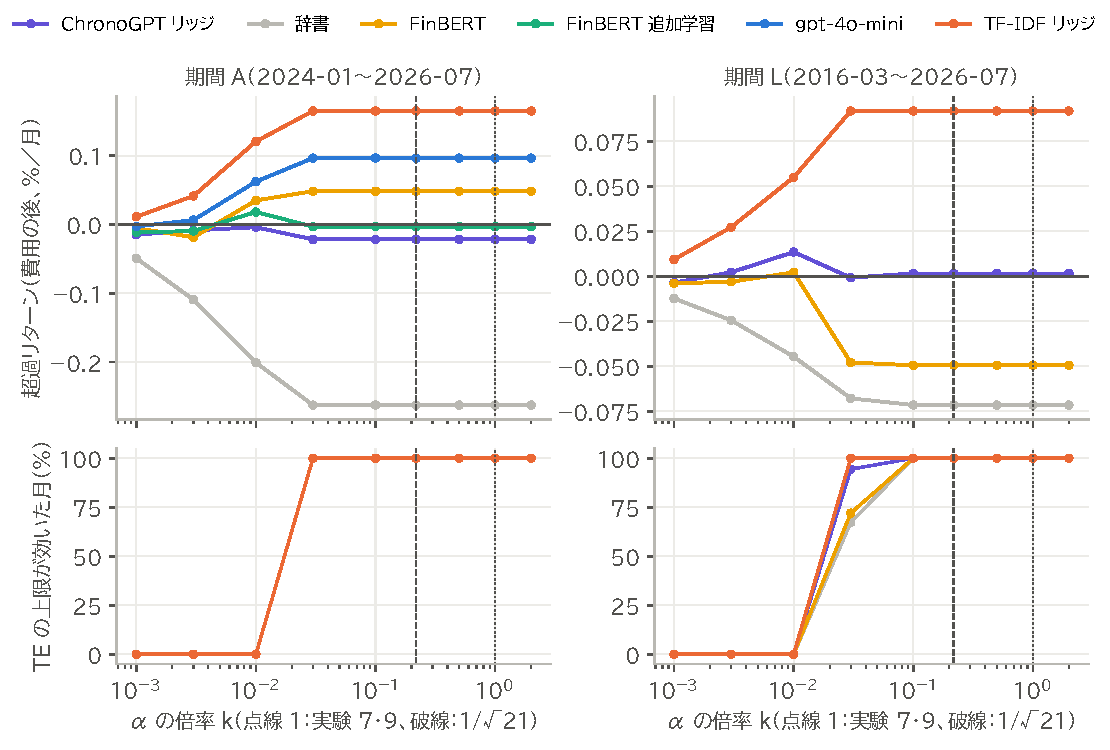
\includegraphics[width=\linewidth]{scale.pdf}
\caption{上：費用の後の月次の超過リターン。下：TE の上限が効いた月の割合。横軸は倍率 $k$（対数）。点線は実験 7・9（$k=1$）、破線は期間に合った大きさ（$k=1/\sqrt{21}$）。}
\label{fig:scale}
\end{figure}

\begin{itemize}
\item $k\geq0.03$（期間 L の一部は $k\geq0.1$）では、TE の上限が毎月効き、どの点数でも成績が 1 桁も違わず同じだった（\figref{fig:scale} の右側の平らな線）。
\item $k\leq0.01$ では上限が効かなくなり、時価総額からのずれはほぼ $k$ に比例して小さくなる。gpt-4o-mini の事前の TE は、$k=0.01$ で 1.47\%、$k=0.001$ で 0.22\%（上限は 1.95\%）。成績も 0 に近づく。
\end{itemize}

\section{なぜ同じになるか}

時価総額の比率を $w_m$、そこからのずれを $x$ とする。均衡リターンは $\Pi=\delta\Sigma w_m$ なので、最適化の目的の $\Pi$ の部分は打ち消し合い、
\[
\max_x\; k\,a'x - \frac{\delta}{2}x'\Sigma x \quad\text{（ただし } x'\Sigma x\le \mathrm{TE}^2\text{、空売りなし）}
\]
になる（$a$ は見通しの向き）。上限が効いているときは $x'\Sigma x=\mathrm{TE}^2$ で一定なので、答えは「$a'x$ を最大にする $x$」で決まり、$k$ によらない。上限が効かなくなる境目は $k\approx0.02$ で、期間に合った大きさ（0.218）はその 10 倍以上大きい。

\begin{verdict}
\textbf{$\alpha$ の単位の誤りは、実験 7・9 の結論に影響しない。}この BLM では、比率は見通しの向きと TE の上限だけで決まる。$\alpha$ の大きさより、TE の上限の決め方（補足実験 X03）のほうが成績を左右する。
\end{verdict}

\section{LLM と NLP の比較}

\begin{figure}[H]
\centering
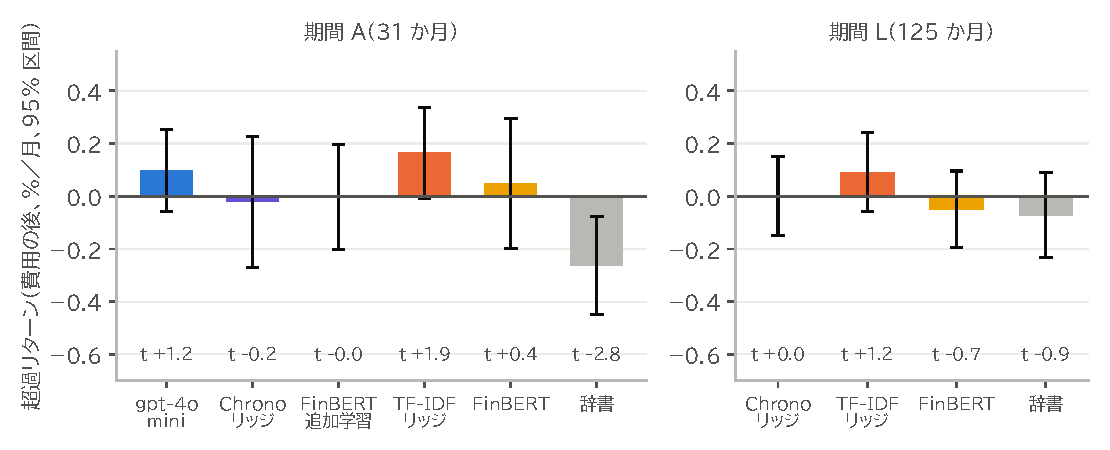
\includegraphics[width=\linewidth]{signals.pdf}
\caption{TE の上限が効く倍率（どの $k\geq0.03$ でも同じ）での、費用の後の月次の超過リターン（95\% 区間）と Newey--West の $t$。}
\label{fig:signals}
\end{figure}

\begin{table}[H]
\centering
\caption{費用の後の月次の超過リターン（対 時価総額）。}
\small
\begin{tabular}{lrr}
\toprule
点数 & 期間 A（31 か月） & 期間 L（125 か月） \\
\midrule
gpt-4o-mini & $+0.10\%$（$t$ 1.2） & — \\
ChronoGPT のリッジ & $-0.02\%$（$t$ $-0.2$） & $+0.00\%$（$t$ 0.0） \\
FinBERT の追加学習 & $-0.00\%$（$t$ $-0.0$） & — \\
TF-IDF＋リッジ & $+0.17\%$（$t$ 1.9） & $+0.09\%$（$t$ 1.2） \\
FinBERT（学習なし） & $+0.05\%$（$t$ 0.4） & $-0.05\%$（$t$ $-0.7$） \\
辞書 & $-0.26\%$（$t$ $-2.8$） & $-0.07\%$（$t$ $-0.9$） \\
\bottomrule
\end{tabular}
\end{table}

\begin{itemize}
\item 費用の後で有意にプラスの点数はない。10 通りを比べているので、$|t|$ 2 前後は偶然でも出うる。辞書の期間 A の $-2.8$ も、10 通りの補正（Holm）をすると有意でない。
\item \textbf{反応の説明力と、月次の成績の並びは一致しない。}発表への 2 日の反応を一番よく説明したのは gpt-4o-mini だった（実験 3〜5、10）。月次の BLM では、単語の出方の TF-IDF のほうが、どちらの期間でも高かった（有意でない）。月末の時点では決算の情報の大部分がもう株価に入っている（実験 8）ので、残りは小さく、どの点数でもほぼ雑音と考えられる（\figref{fig:signals}）。
\end{itemize}

% ============================================================
\chapter{まとめと限界}\label{ch:summary}

\begin{enumerate}
\item 実験 7・9 の「月次の BLM は市場とほぼ同じ」は、$\alpha$ の大きさの設定のせいではない。
\item この BLM では TE の上限がほぼ常に効くので、見通しの大きさではなく向きだけが比率を決める。実務でも、TE の上限を置く BLM では同じことが起きる。
\item 決算の点数は、LLM でも NLP でも、月次では効かない。
\end{enumerate}

\textbf{限界}：実験 7・9 の結果を見た後の分析で、事前登録はしていない。期間 A は 31 か月しかない。倍率の 0.001〜0.03 は、1 回目の結果を見て足した。

% ============================================================
\chapter*{再現の手順}
\addcontentsline{toc}{chapter}{再現の手順}

\begin{verbatim}
python experiments/X05_alpha_scale/run.py          # k = 0.1 .. 2
python experiments/X05_alpha_scale/run.py small    # k = 0.001 .. 0.03
cd 資料集/02_実験/補足実験_αの大きさ
python 作成スクリプト/figs.py                       # この資料の図
\end{verbatim}

数値の出どころは \code{experiments/X05\_alpha\_scale/results/} の \code{summary.csv}、\code{small/summary.csv}、\code{findings.md}。費用は 0 円（CPU で約 40 分）。

\end{document}
